\title{Year 12 Chemistry Depth Study}
\author{
NESA \#: 34364338 
}

\documentclass[12pt, a4paper]{article}
\usepackage[margin=0.5in]{geometry}
\usepackage{parskip}
\usepackage{amsmath}
\usepackage{float}
\usepackage[T1]{fontenc}

\hyphenpenalty 10000
\exhyphenpenalty 10000

\usepackage{graphicx}
\graphicspath{ {./images/} }

\begin{document}
\maketitle





\section{Equilibrium Systems: Contact Process}

The Contact Process is a multi-step industrial process used to produce concentrated sulfuric acid. 

\begin{enumerate}
	\item Produce sulfur dioxide from sulfur and excess oxygen
	\item Convert sulfur dioxide to sulfur trioxide
	\item Produce oleum (fuming sulfuric acid) from sulfur trioxide
	\item React oleum with water to produce concentrated sulfuric acid
\end{enumerate}

The key equilibrium reaction is the conversion of sulfur dioxide to sulfur trioxide, an exothermic reversible reaction.

\begin{align}
	2SO_{2}(g) + O_{2} \rightleftharpoons 2SO_{3}(g) \qquad \qquad \Delta H = -196 \; kJ \; mol^{-1}
\end{align}


\subsection{The importance and uses of sulfuric acid}

Sulfuric acid is a key primary product used to produce a number of other chemical compounds, and the Contact Process allows them to be produced efficently in high concentrations at industrial scales. 

\subsubsection{Fertilisers}
Sulfuric acid is a key reactant for the production of phosphate-based fertilisers. For example, calcium phosphates are often used as fertiliser and is produced by reacting phosphorite with sulfuric acid.

\begin{align}
	Ca_{3}(PO_{4})_{2}(s) + H_{2}SO_{4}(aq) \rightarrow Ca(H_{2}PO_{4})_{2}(s) + 2CaSO_{4}(s)
\end{align}

Phosphate-based fertilisers are critical to the world's food supply, in ensuring that there is enough food production to sustain a growing world population. According to researchers, without phosphate and nitrogen-based fertilisers, humanity would only be able to produce half its current food production (Faradji \& de Boer, 2016.)

\subsubsection{Cleaning agents}
Outside of fertiliser, sulfuric acid is also used as an industrial cleaning agent. It helps to remove oxidation and rust from iron and steel-based components in the passenger motor vehicles (PMV) and major appliances industries, while also featuring as an ingredient in some household cleaning agents such as drain cleaners.


\subsection{Factors affecting equilibrium}

\textbf{Le Chatelier's Principle} states that within equilibrium, a disturbance caused by changing conditions (such as temperature, pressure and concentration) will result in an \textbf{equilibrium shift} to counteract and re-establish the equilibrium. In the case of the Contact Process, it features one \textbf{equilibrium reaction}: the conversion of sulfur dioxide to sulfur trioxide.

\begin{align}
	2SO_{2}(g) + O_{2} \rightleftharpoons 2SO_{3}(g) \qquad \qquad \Delta H = -196 \; kJ \; mol^{-1}
\end{align}






\subsubsection{Temperature}

The forward reaction is \textbf{exothermic} (\(\Delta H = -196 \; kJ \: mol^{-1}\)). By \textbf{Le Chatelier's Principle}, lowering temperature will favour the exothermic side of the reaction. Hence, as temperature decreases, the equilibrium shifts right and the disturbance of the equilibrium is counteracted by an increase in the production of sulfur trioxide. Therefore, the ideal condition for optimal yield would be a temperature of 0°C. However, as temperature decreases, there is less kinetic energy and less frequent successful collisions, hence the rate of reaction decreases (as increased energy is required to break bonds). As demonstrated in the provided graph, this temperature has its highest yield between 0°C (100\%) and 400°C (80\%), with minimal yield changes as temperature approaches zero from 400°C. At higher temperatures above 400°C, the change in the percentage conversion rate is more significant. As a result, to produce a reasonably high yield while maintaing a fast rate, a higher compromise temperature of \textbf{400°C to 450°C} is often used in industrial applications. This compromise temperature is chosen to ensure that a relatively high yield of sulfur trioxide can be formed, while ensuring the rate of reaction remains relatively high.

\begin{center}
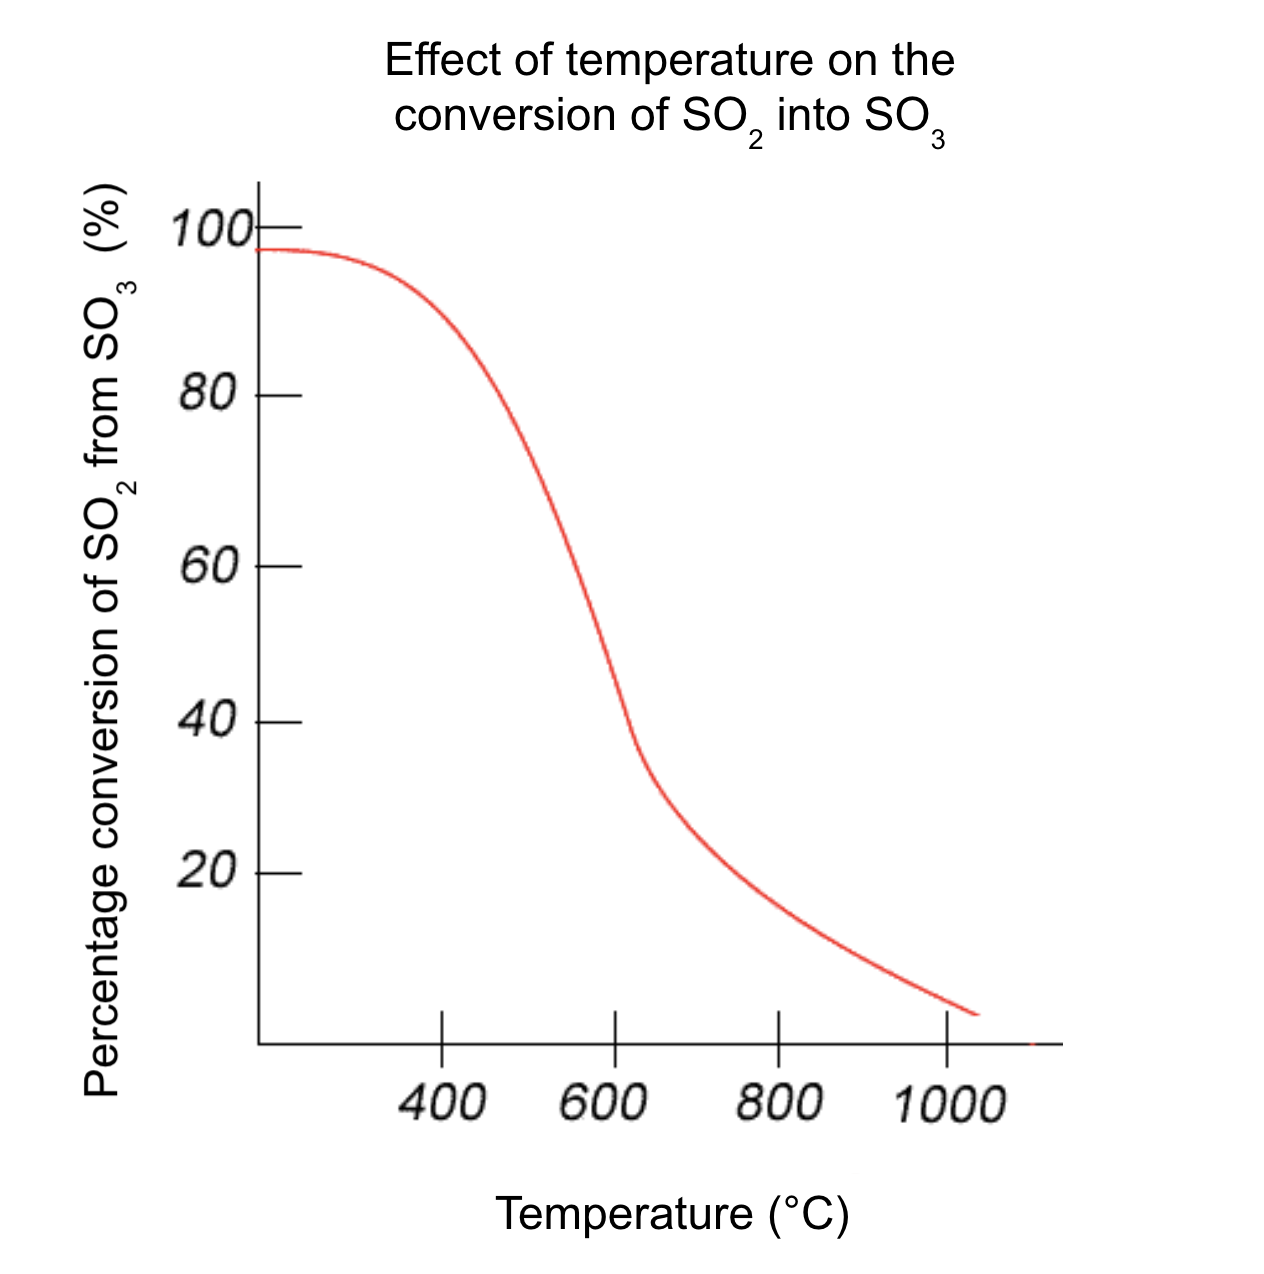
\includegraphics[scale=0.5]{graph}
\\
\textbf{Figure 1:} Temperature/yield graph for the conversion of \(SO_{2}\) into \(SO_{3}\)
\end{center}






\subsubsection{Pressure}

By \textbf{Le Chatelier's Principle}, an increase in pressure will favour the side with fewer number of moles. In the equilibrium reaction, this is the products side, and the equilibrium shifts right. The system will then counteract the disturbance by decreasing pressure, which will produce more sulfur trioxide. Increasing pressure will also increase the amount of kinetic energy, hence increasing the frequency of successful collisions, and hence increasing the rate of reaction.

However, in industrial applications, lower pressures are used at around 1 to 2 atm, as they still generate high yield (99.5\%) and often it is economically not justifiable to invest in substantially higher pressures for minimal yield gain. There are also considerable safety risks associated with high pressure equipment, particularly in times of failure, where fragmentation or disruption of equipment could cause human injury.






\subsubsection{Concentration}

By \textbf{Le Chatelier's Principle}, an increase in reactants will disturb equilibrium. Initially, the forward rate increases sharply given a sudden increase in the amount of reactants, before the forward rate decreases (and the reverse rate increases) gradually to approach a constant rate but higher equilibrium, resulting in a net forward reaction due to a higher number of molecules resulting in an increased collision frequency. A shift to the right occurs and there is the production of more sulfur trioxide. Hence, an increase in the concentration of reactants will result in a shift to the right. 

Hence, an optimal yield would be gained by increasing the amount of reactants as far as possible. In industrial applications, oxygen and sulfur dioxide is often used in a 1:1 ratio such that oxygen will always remain in excess, thus allowing for a consistent right shift while maintaining the rate of reaction.





\subsubsection{Catalyst}

\textbf{Catalysts} lower the activation energy required for the reaction to take place, increasing the rate of reaction. By lowering the activation energy, the bonds in the reactants weaken, thereby increasing the rate of reaction, and eliminating the need for otherwise-needed expensive high-pressure systems. 

Within the equilibrium reaction, a catalyst of vanadium(V) oxide (\(V_{2}O_{5}\)) is used for a reversible reaction, enabling a dynamic equilibrium to be established. Without a catalyst, the reaction would virtually remain at a static equilibrium.






\section{Industrial Design: Solvay Process}

\subsection{Exploring the Solvay Process}

The Solvay Process is a synthesis reaction which reacts carbon dioxide (produced from limestone), ammonia and brine to produce sodium carbonate, as represented in the following flowchart:

\begin{center}
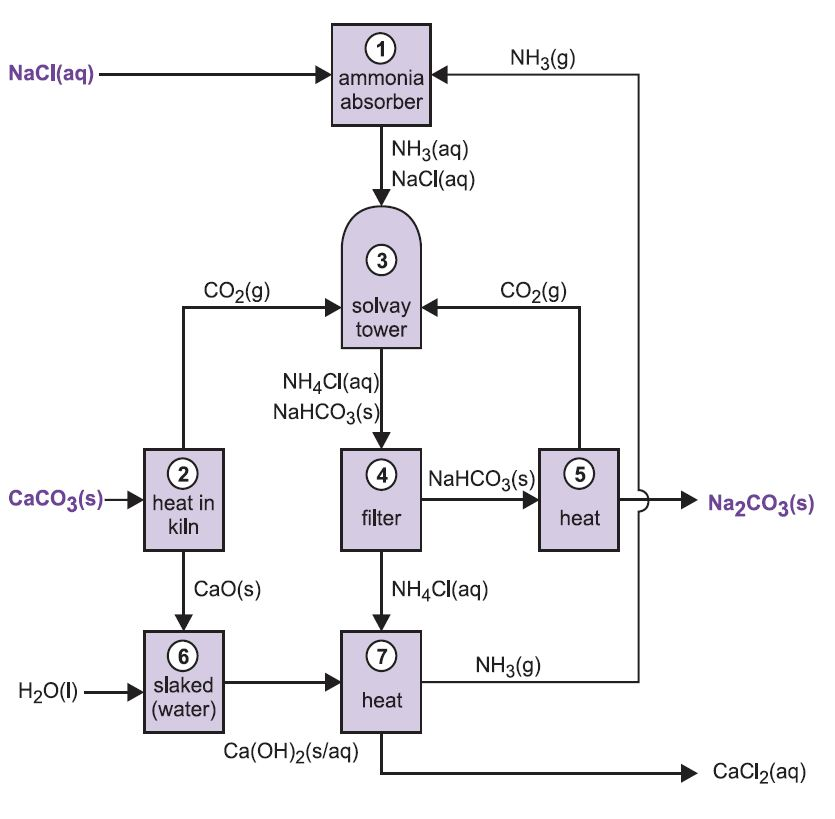
\includegraphics[scale=0.6]{solvay.jpeg}
\\
\end{center}




\subsubsection{Ammonia gas as a reactant}

Brine (\(NaCl(aq)\)) is fed through an ammonia absorber at (1), where \(NH_{3}(aq)\) is added to the reactants. The \(NH_{3}(aq)\) used is often recycled in high proportions in later stages at (7).

\begin{align}
	Ca(OH)_{2}(s) + 2NH_{4}Cl(aq) \rightarrow 2NH_{3}(g) + CaCl_{2}(aq) + 2H_{2}O(l) \qquad \Delta H = -20 \; kJ \; mol^{-1}
\end{align}


\subsubsection{The effect of heating calcium carbonate}

Coke burns in a counter-current of pre-heated oxygen gas, heating the kiln to at least 840°C. This process is \textbf{exothermic} (with a negative enthalpy change).

\begin{align}
	C(s) + O_{2}(g) \rightarrow CO_{2}(g) \qquad \Delta H = -65 \; kJ \; mol^{-1}
\end{align}

Hence, there will be enough energy to establish a dynamic equilibrium, enabling the subsequent calcination (thermal decomposition) of calcium carbonate (limestone), which is an endothermic process with positive enthalpy change depicted at (2).

\begin{align}
	CaCO_{3}(s) + heat \rightleftharpoons CaO(s) + CO_{2}(g) \qquad \qquad \Delta H = +178 \; kJ \; mol^{-1}
\end{align}

\subsubsection{Solvay tower}

The key equilibrium reaction at (3) involves saturating brine (sodium chloride solution) with ammonia gas and carbon dioxide to form ammonium chloride and sodium bicarbonate. At low temperatures, the reaction shifts right towards the exothermic products side of the reaction. Thermal pollution from exothermic Solvay reactions remains an ongoing environmental concern.

\begin{align}
	NaCl(aq) + NH_{3}(aq) + H_{2}O(l) + CO_{2}(g) \rightleftharpoons NH_{4}Cl(aq) + NaHCO_{3}(s)  \qquad \Delta H = -158 \; kJ \; mol^{-1}
\end{align}

\subsubsection{Forming sodium carbonate}

At (4), aqueous ammonia chloride is filtered from solid sodium bicarbonate. 

Sodium bicarbonate is then heated (and hence dehydrated) at (5) in order to produce sodium carbonate, and will begin to thermally decompose at around 100°C, with complete conversion at 200°C (Senese, 2010).

\begin{align}
	2NaHCO_{3}(s) + heat \rightleftharpoons Na_{2}CO_{3}(s) + H_{2}O(g) + CO_{2}(g) \qquad \Delta H = +85 \; kJ \; mol^{-1}
\end{align}


\subsubsection{Recycling calcium oxide to form ammonia gas}

In the calcination reaction, calcium oxide is also produced alongside carbon dioxide. This can be used to form and hence recycle ammonia gas. It is first reacted with water to form calcium hydroxide in a process known as \textbf{slaking}, located at (6).

\begin{align}
	CaO(s) + H_{2}O(l) \rightarrow Ca(OH)_{2} \qquad \Delta H = -65 \; kJ \; mol^{-1}
\end{align}

Calcium hydroxide is then reacted and heated with the produced ammonium chloride \(NH_{4}Cl\) from the Solvay equilibrium reaction, to form ammonia gas, calcium chloride and water at (7).


\subsection{Risk assessment}

\begin{table}[H]
	\centering
\begin{tabular}{|p{5cm}|p{12cm}|}
	\hline
\textbf{Hazard}                    & \textbf{Risk}                                                                                                                                                                                                          \\  \hline


Heating of calcium carbonate 	  & Calcium carbonate is heated to upwards 600-800°C. There would be a fire hazard given the presence of flammable material.                                                                                                                                                                                                                                                                        \\  \hline
Corrosiveness, flammability and toxicity of ammonia gas                      & Inhalation of calcium oxide could cause coughing or breathing difficulties or life-threatening pulmonary edema (fluid in the lungs). \\  \hline
Carbon dioxide gas               & Exposure to high concentrations of carbon dioxide gas can lead to drowsiness or nausea. At 5000 ppm and above, this could lead to oxygen deprivation.                                                                                                                                                                                                                \\  \hline
Calcium oxide as an irritant and corrosive waste product & Inhalation of calcium oxide could cause coughing or breathing difficulties or life-threatening pulmonary edema (fluid in the lungs).  \\  \hline
Calcium hydroxide                & Skin contact could cause irritation or burning. Eye damage could occur upon eye contact.                                                                                                                                                                                                                                                                                                                   \\  \hline
Ammonium chloride as an irritant              & Inhaling ammonium chloride fumes may induce coughing or breathing difficulties.

\\ \hline                                                 

\end{tabular}
\end{table}

\pagebreak

\subsection{Assessment of key considerations}

This section assesses the relevant key economical, environmental and social considerations applicable to the Solvay Process at Penrice Factory, Osborne SA, operational from 1935 to 2014.

\subsubsection{Economical}

\paragraph{Advantages}
Penrice Factory is in close proximity to key resources and materials, including the Port River, the St Kilda salt lagoons, the Osborne Power Station, and the Penrice limestone quarry in the Barossa Valley. Being located in Adelaide, it could take advantage of a large local supply of labour, with sufficient housing and access to public services and railway lines.

\paragraph{Disadvantages}

Being located within Australia, Penrice Factory was vulnerable to foreign imports, over-reliance on the Australian dollar, increased regulation, and increased taxes (particularly the 2011-2014 carbon tax). It's inability to compete against cheaper foreign imports in addition to the carbon tax resulted in the factory's closure in 2014.

\subsubsection{Environmental}

\paragraph{Advantages}
Penrice Factory recycles ammonia and carbon dioxide, such that only small amounts of ammonia need to be refilled at intervals. This somewhat mitigates the impact on the nearby Port River Estuary by reusing waste products. 

\paragraph{Disadvantages}
Penrice Factory is one of the main sources of oxidised nitrogen and ammonia being present within the Port River Estuary (Environment Protection Authority, 2003). Other outflow includes calcium chloride and nitrogen. High nutrient concentrations leads to excessive algae and plant growth, cause fish deaths, or suffocate seagrass. Furthermore, outflow from the factory is responsible for thermal pollution of the estuary, given that the Solvay process is largely exothermic. 

\subsubsection{Social}

\paragraph{Advantages}
Penrice Factory has been operating for 80 years. At the time of its closure, there were 95 employees at the plant. It also acted as major demand source for the nearby Penrice quarry, with 180 employees across the former Penrice Soda Products corporation.

\begin{center}
\includegraphics[scale=0.3]{earth}
\\
\end{center}

\paragraph{Disadvantages}

The Penrice Factory stockpiled large amounts of calcium carbonate on land after EPA action against their dumping in the Port River. Large mounds of calcium carbonate were considered to be an "eyesore" by residents and blocked views of the Port River. 

Penrice Factory was also responsible for a considerable number of noise complaints, especially during plant slowdowns, startups, and maintenance exercises.

\subsubsection{Justification for location suitability}

Although there are many economic advantages of the site (including its close proximity to key resources) its impact on the environment and surrounding community has been largely devastating. This includes it being a major factor towards the the Port River Estuary's poor to moderate water quality, a result of decades of nutrient pollution, thermal pollution and human impact. Furthermore, while it contributed to local jobs, it had a largely negative impact for urban areas of metropolitan Adelaide, in the form of noise \& dust pollution, and visually undesirable stockpiled calcium carbonate waste product. Therefore, the Penrice Factory is located in a largely unsuitable location due to its social and environmental impacts to the surrounding community. 
\pagebreak

\section{Bibliography}

British Broadcasting Corporation 2021, Sulfuric acid and the contact process, viewed 17 October 2021, \\ \textless{https://www.bbc.co.uk/bitesize/guides/zb7f3k7/revision/1}\textgreater

Canadian Centre for Occupational Health and Safety, Ammonia, viewed 31 October 2021, \\ \textless{https://www.ccohs.ca/oshanswers/chemicals/chem\_profiles/ammonia.html}\textgreater

Clark, Jim 2021, \emph{The Contact Process}, Truro School in Cornwall, viewed 17 October 2021, \\ \textless{https://chem.libretexts.org/@go/page/3838}\textgreater

Department of Agriculture, Water and the Environment 2019, Sulfuric acid, Commonwealth of Australia, viewed 18 October 2021, \textless{http://www.npi.gov.au/resource/sulfuric-acid}\textgreater

Dynamic Science n.d., Sulfuric acid - contact process, viewed 1 November 2021, \textless{http://www.dynamicscience.com.au/tester/solutions1/chemistry/sulfuricacid.html}\textgreater (Figure 1)

Faradji, Charly \& de Boer, Marissa 2016, \emph{How the great phosphorus shortage could leave us all hungry}, The Conversation, viewed 18 October 2021, \\ \textless{https://theconversation.com/how-the-great-phosphorus-shortage-could-leave-us-all-hungry-54432}\textgreater

IB Chemistry Web 2016, Equilibrium: Industrial Processes 2016, viewed 22 October 2021, \\ \textless{https://www.ibchem.com/IB16/07.27.htm}\textgreater

Manahan, S E 2016, \emph{Industrial Chemical Reactions - The Solvay Process}, University of Missouri, viewed 24 October 2021 \\ \textless{https://chem.libretexts.org/@go/page/285417}\textgreater

Millington, L \& Bazeley, T, \emph{Proposed development and construction of housing for Defence at Langs North (Bayriver, Port Adelaide, South Australia}, Port Adelaide Residents Environment Protection Group Inc, viewed 2 November 2021 \\ \textless{https://www.aph.gov.au/parliamentary\_business/committees/house\_of\_representatives\_committees?url=pwc/largsnorth/subs/sub03.pdf}\textgreater

New Jersey Department of Health 2016, Right to Know Hazardous Substance Fact Sheet: Ammonium Chloride, viewed 31 October 2021, \\ \textless{https://www.nj.gov/health/eoh/rtkweb/documents/fs/0093.pdf}\textgreater

New Jersey Department of Health and Senior Services 2003, Hazardous Substance Fact Sheet: Calcium Oxide, viewed 31 October 2021, \\ \textless{https://nj.gov/health/eoh/rtkweb/documents/fs/0325.pdf}\textgreater

Penrice Soda Holdings Limited 2007, Annual Report 2007, viewed 2 November 2021, \\ \textless{https://www.asx.com.au/asxpdf/20070928/pdf/314v1zngpdyll1.pdf}\textgreater

Royal Society of Chemistry n.d., Part 4: Manufacturing sodium carbonate by the Solvay process, viewed 29 October 2021, \\ \textless{https://edu.rsc.org/download?ac=15607}\textgreater

Royal Society of Chemistry n.d., Part 5: The thermodynamics and equilibria involved in the Solvay process for producing sodium carbonate, viewed 29 October 2021, \\ \textless{https://edu.rsc.org/download?ac=15610}\textgreater

Science Learning Hub 2021, Carbonate chemistry, viewed 31 October 2021, \\ \textless{https://www.sciencelearn.org.nz/resources/469-carbonate-chemistry}\textgreater

Senese, Fred 2010, \emph{What happens when sodium bicarbonate is headed?}, General Chemistry Online! (Frostburg State University's Department of Chemistry), \\ \textless{https://antoine.frostburg.edu/chem/senese/101/inorganic/faq/carbonate-decomposition.shtml}\textgreater

South Australia Environment Protection Authority 2003, Water Quality of the Port River Estuary – a community summary, viewed 2 November 2021, \\ \textless{https://www.epa.sa.gov.au/files/8636\_wq\_portriver.pdf}\textgreater

The Advertiser 2013, Penrice to shut soda ash manufacturing at Osborne plant in South Australia, impacting 60 jobs, viewed 2 November 2021, \\ \textless{https://www.adelaidenow.com.au/news/penrice-to-shut-soda-ash-manufacturing-at-osborne-plan-in-south-australia-impacting-60-jobs/news-story/ecae8b19856bd02ead367a181515f382}\textgreater

The Essential Chemistry Industry 2016, Sulfuric acid, viewed 18 October 2021, \\ \textless{https://www.essentialchemicalindustry.org/chemicals/sulfuric-acid.html}\textgreater

Vedantu, Contact Process n.d., viewed 22 October 2021, \\ \textless{https://www.vedantu.com/iit-jee/contact-process}\textgreater

Wansbrough, H \& Simpson, J \& Petherick, J \& Donaldson, L 2017, \emph{The Manufacture of Sulfuric Acid and Superphosphate}, New Zealand Institute of Chemistry, viewed 24 October 2021, \\ \textless{https://nzic.org.nz/app/uploads/2017/10/1B.pdf}\textgreater

Wisconsin Department of Health Services 2021, Carbon Dioxide, viewed 31 October 2021, \\ \textless{https://www.dhs.wisconsin.gov/chemical/carbondioxide.htm}\textgreater

Wikipedia contributors 2021, \emph{Contact process}, Wikipedia, the Free Encyclopedia, viewed 22 October 2021, \\ \textless{https://en.wikipedia.org/w/index.php?title=Contact\_process\&oldid=1047723670}\textgreater

Wikipedia contributors 2021, \emph{Penrice Soda Products}, Wikipedia, the Free Encyclopedia, viewed 1 November 2021, \\ \textless{https://en.wikipedia.org/w/index.php?title=Penrice\_Soda\_Products\&oldid\=1022061942}\textgreater

World of Chemicals 2021, Manufacturing of sodium carbonate by solvay process, viewed 31 October 2021, \\ \textless{https://www.worldofchemicals.com/440/chemistry-articles/manufacturing-of-sodium-carbonate-by-solvay-process.html}\textgreater

\end{document}

==================================================

inline notes:

- are we doing solvay process?
- manually use bibliography because the high school is too basic for bibtex :( - no Harvard AU support + they don't like [n]
- format date{today} later 
- check contact process concentration
- cut down word count


- economic disadvantage: producing CaCl2

- overall equation
- ionic equiations 
